\documentclass[11pt,a4paper]{article}
\usepackage{fontspec}
\setmainfont{TeX Gyre Pagella}
\newfontfamily\headfont{Inter}[UprightFont=*-ExtraBold,BoldFont=*-ExtraBold,Extension=.otf,Path=/usr/share/fonts/opentype/inter/]
\usepackage[a4paper,margin=2.3cm]{geometry}
\usepackage{graphicx,booktabs,float,caption,array,xcolor,longtable}
\usepackage{xurl}
\usepackage[hidelinks]{hyperref}
\usepackage{titlesec}
\usepackage[round]{natbib}
\usepackage{setspace}
\setstretch{1.05}
\renewcommand{\topfraction}{0.9}
\renewcommand{\bottomfraction}{0.8}
\renewcommand{\textfraction}{0.1}
\renewcommand{\floatpagefraction}{0.75}
\setlength{\parindent}{0pt}
\setlength{\parskip}{0.55em}
\titleformat{\section}{\headfont\Large}{\thesection}{0.8em}{}
\titleformat{\subsection}{\headfont\large}{\thesubsection}{0.8em}{}
\captionsetup{font=small,labelfont=bf}
\urlstyle{same}
\hypersetup{pdftitle={Lighthouses of the World},pdfauthor={Tristan Hotham}}

\begin{document}
\begin{center}
{\Large\bfseries Lighthouses of the World\par}
\vspace{0.4em}
{\large Where they stand, when they were built, the oldest and the tallest:\\9,770 lighthouses in Wikidata, measured against the length of the coast\par}
\vspace{1.2em}
{\large Tristan Hotham\par}
\vspace{0.3em}
{\small Independent researcher\\
ORCID: 0000-0003-4931-9349\\
DOI: https://doi.org/10.5281/zenodo.23857614\par}
\vspace{0.8em}
2026
\end{center}

\begin{quote}
\small
\begin{center}\textbf{Abstract}\end{center}
I map every lighthouse in Wikidata that has coordinates, 9,770 after removing keepers' houses and replicas, and measure the lights against the length of each country's sea coast on Natural Earth's 1:10m map. Wikidata dates 6,546 of them. Building follows the industrial century: outside Sweden, new lights rise from 103 in the 1820s to a peak of 376 in the 1870s, stay above three hundred a decade until the First World War and then fall, to about 97 a decade from 1970 to 2019, a decline that coincides with automation and satellite navigation. Sweden's 2,555 lights, 26\% of the total, show a second, twentieth-century wave of small lights that peaks in the 1940s, which I read as the trace of a national list loaded in full. Per 1,000 km of coast, Sweden (341) and Finland (126) lead, against 9.4 for the world; all ten densest regional coasts are Swedish or Finnish, and outside those two countries Lower Saxony and Connecticut lead. The oldest dated lighthouse still standing is the Tower of Hercules, dated AD~100; the tallest traditional tower, from Wikipedia's list, is the Île Vierge lighthouse at 83~m. Coverage is very uneven: 60\% of the lights have at most one Wikipedia article, and some coastal countries have none in Wikidata. The map is as much a map of the record as of the sea.

\textbf{Keywords:} lighthouses; maritime history; navigation; Wikidata; coastline length; Natural Earth; open data; coverage bias; mapping
\end{quote}

\section{Introduction}
A lighthouse is a building with a single public purpose: to mark a coast that has killed ships, so that it kills fewer. The oldest that still stand are Roman; the great majority were built in the nineteenth and early twentieth centuries, when iron construction, the Fresnel lens and the growth of steam shipping made it possible, and necessary, to light the world's main coasts systematically. Automation through the twentieth century and satellite navigation at its end changed their role again.

No complete open register of the world's lighthouses exists. National lists of lights are kept by hydrographic offices, and the most complete public directory is the work of one enthusiast \citep{rowlett}. Wikidata \citep{wikidata}, the free knowledge base behind Wikipedia, holds thousands of lighthouses, some added one by one with Wikipedia articles and some loaded in bulk from national lists. This paper uses it to ask four simple questions: where are the lights, relative to how much coast each country has; when were they built; which are the oldest still standing and the tallest; and how far can the record be trusted? An interactive version, with a day map and a ``night glow'' map, is at \url{https://maps.tristanhotham.com/lighthouses/}.

\section{Data}
\textbf{Wikidata.} Every item that is an instance of lighthouse (Q39715) or one of its subclasses and has coordinates (P625), retrieved through the QLever service in 2026, with its English label, number of Wikipedia sitelinks, country (P17), inception (P571), height (P2048) and focal height (P2923). The extract has 11,614 rows, one per combination of values, for 9,810 items. Heights were extracted as amounts without their units, which in Wikidata may be metres or feet.

\textbf{Wikipedia.} The English Wikipedia ``List of tallest lighthouses'' \citep{wikitall}, revision 1306705349, which lists 28 traditional lighthouses (as defined by \citealt{rowlett}) of 60~m or more with height in feet and metres, construction, place and year.

\textbf{Natural Earth.} Countries at 1:10m and 1:50m, states and provinces at 1:10m and populated places \citep{naturalearth}, public domain.

\section{Methods}
\subsection{Cleaning}
I kept one row per item, taking the earliest inception year where there are several (44 items) and all distinct height values. I removed 39 items that are buildings at light stations or modern replicas (labels containing ``keeper'', ``accommodation block'', ``barrack block'' or ``replica'') and 1 item whose coordinates are recorded as unknown, leaving 9,770. 1,799 lights (18\%) have no English label and are identified by their Wikidata number.

\subsection{Countries, sea and inland lights}
Each light is placed in the Natural Earth 1:10m map unit that contains it; for lights on rocks offshore, the nearest unit within 30~km (6,001 lights); beyond that, the country Wikidata gives (97). Map units are used as they are, so dependencies such as Greenland, Puerto Rico and the Faroe Islands count separately; Åland is merged into Finland. The location-based country differs from Wikidata's own statement for 175 lights, mostly territories that Natural Earth maps on their own (Hong Kong, Puerto Rico), disputed areas, and offshore lights near a border; country assignment follows Natural Earth's boundaries throughout. A light on land more than 5~km from the sea coast (below) is a lake or river light: 1,075 of them (11\%), mostly on the Great Lakes and the lakes of Sweden and Finland. They are counted in the totals but not in the per-coast figures.

\subsection{Coast length}
Natural Earth's standard country polygons include lakes, so a country's outline consists of its sea coast and its land borders. I take each country's 1:10m outline, remove the parts within about 300~m of any neighbouring country, and measure what remains on the WGS84 ellipsoid. The same procedure on the 1:10m states and provinces gives regional coasts. The world total at this scale is 921,367~km. Coastline length depends on the scale of measurement \citep{mandelbrot}: at 1:10m, fjords, skerries and small islands are smoothed or missing, so these lengths compare places on a common footing but are not true lengths. Densities are given for countries with at least 1,000 km of coast and 10 sea lights and for regions with at least 150 km of coast and 15 sea lights.

\subsection{Oldest and tallest}
Dates are Wikidata's inception years as given; many early dates are rounded and often refer to the first light on the site rather than the present tower. Wikidata's ``still standing'' status is not part of the extract, so for the 17 best known of the oldest lights I marked by hand, from their published histories and the Wikipedia list, whether the tower stands, was rebuilt or is lost; others are marked ``not checked''. Because heights lack units, I rank the tallest from the Wikipedia list only, and use Wikidata heights only to test how often they are in feet.

\section{Results}
\subsection{Where}
Table~\ref{tab:countries} and Figure~\ref{fig:countries} give the counts. Sweden has 2,555 lights, the United States 923, Finland 794, Canada 473 and the United Kingdom 468; the top three hold 44\% of the total. 162 countries and territories have at least one. Per 1,000~km of coast, Sweden (340.6) and Finland (125.5) are far ahead of Tunisia (85.1) and Germany (71.4); France (48.4), Spain (46.8) and the United Kingdom (39.0) are close together. The lowest densities belong to countries with very long coasts: Canada 2.9, Russia 1.2 and Indonesia 0.2.

\begin{figure}[tbp]\centering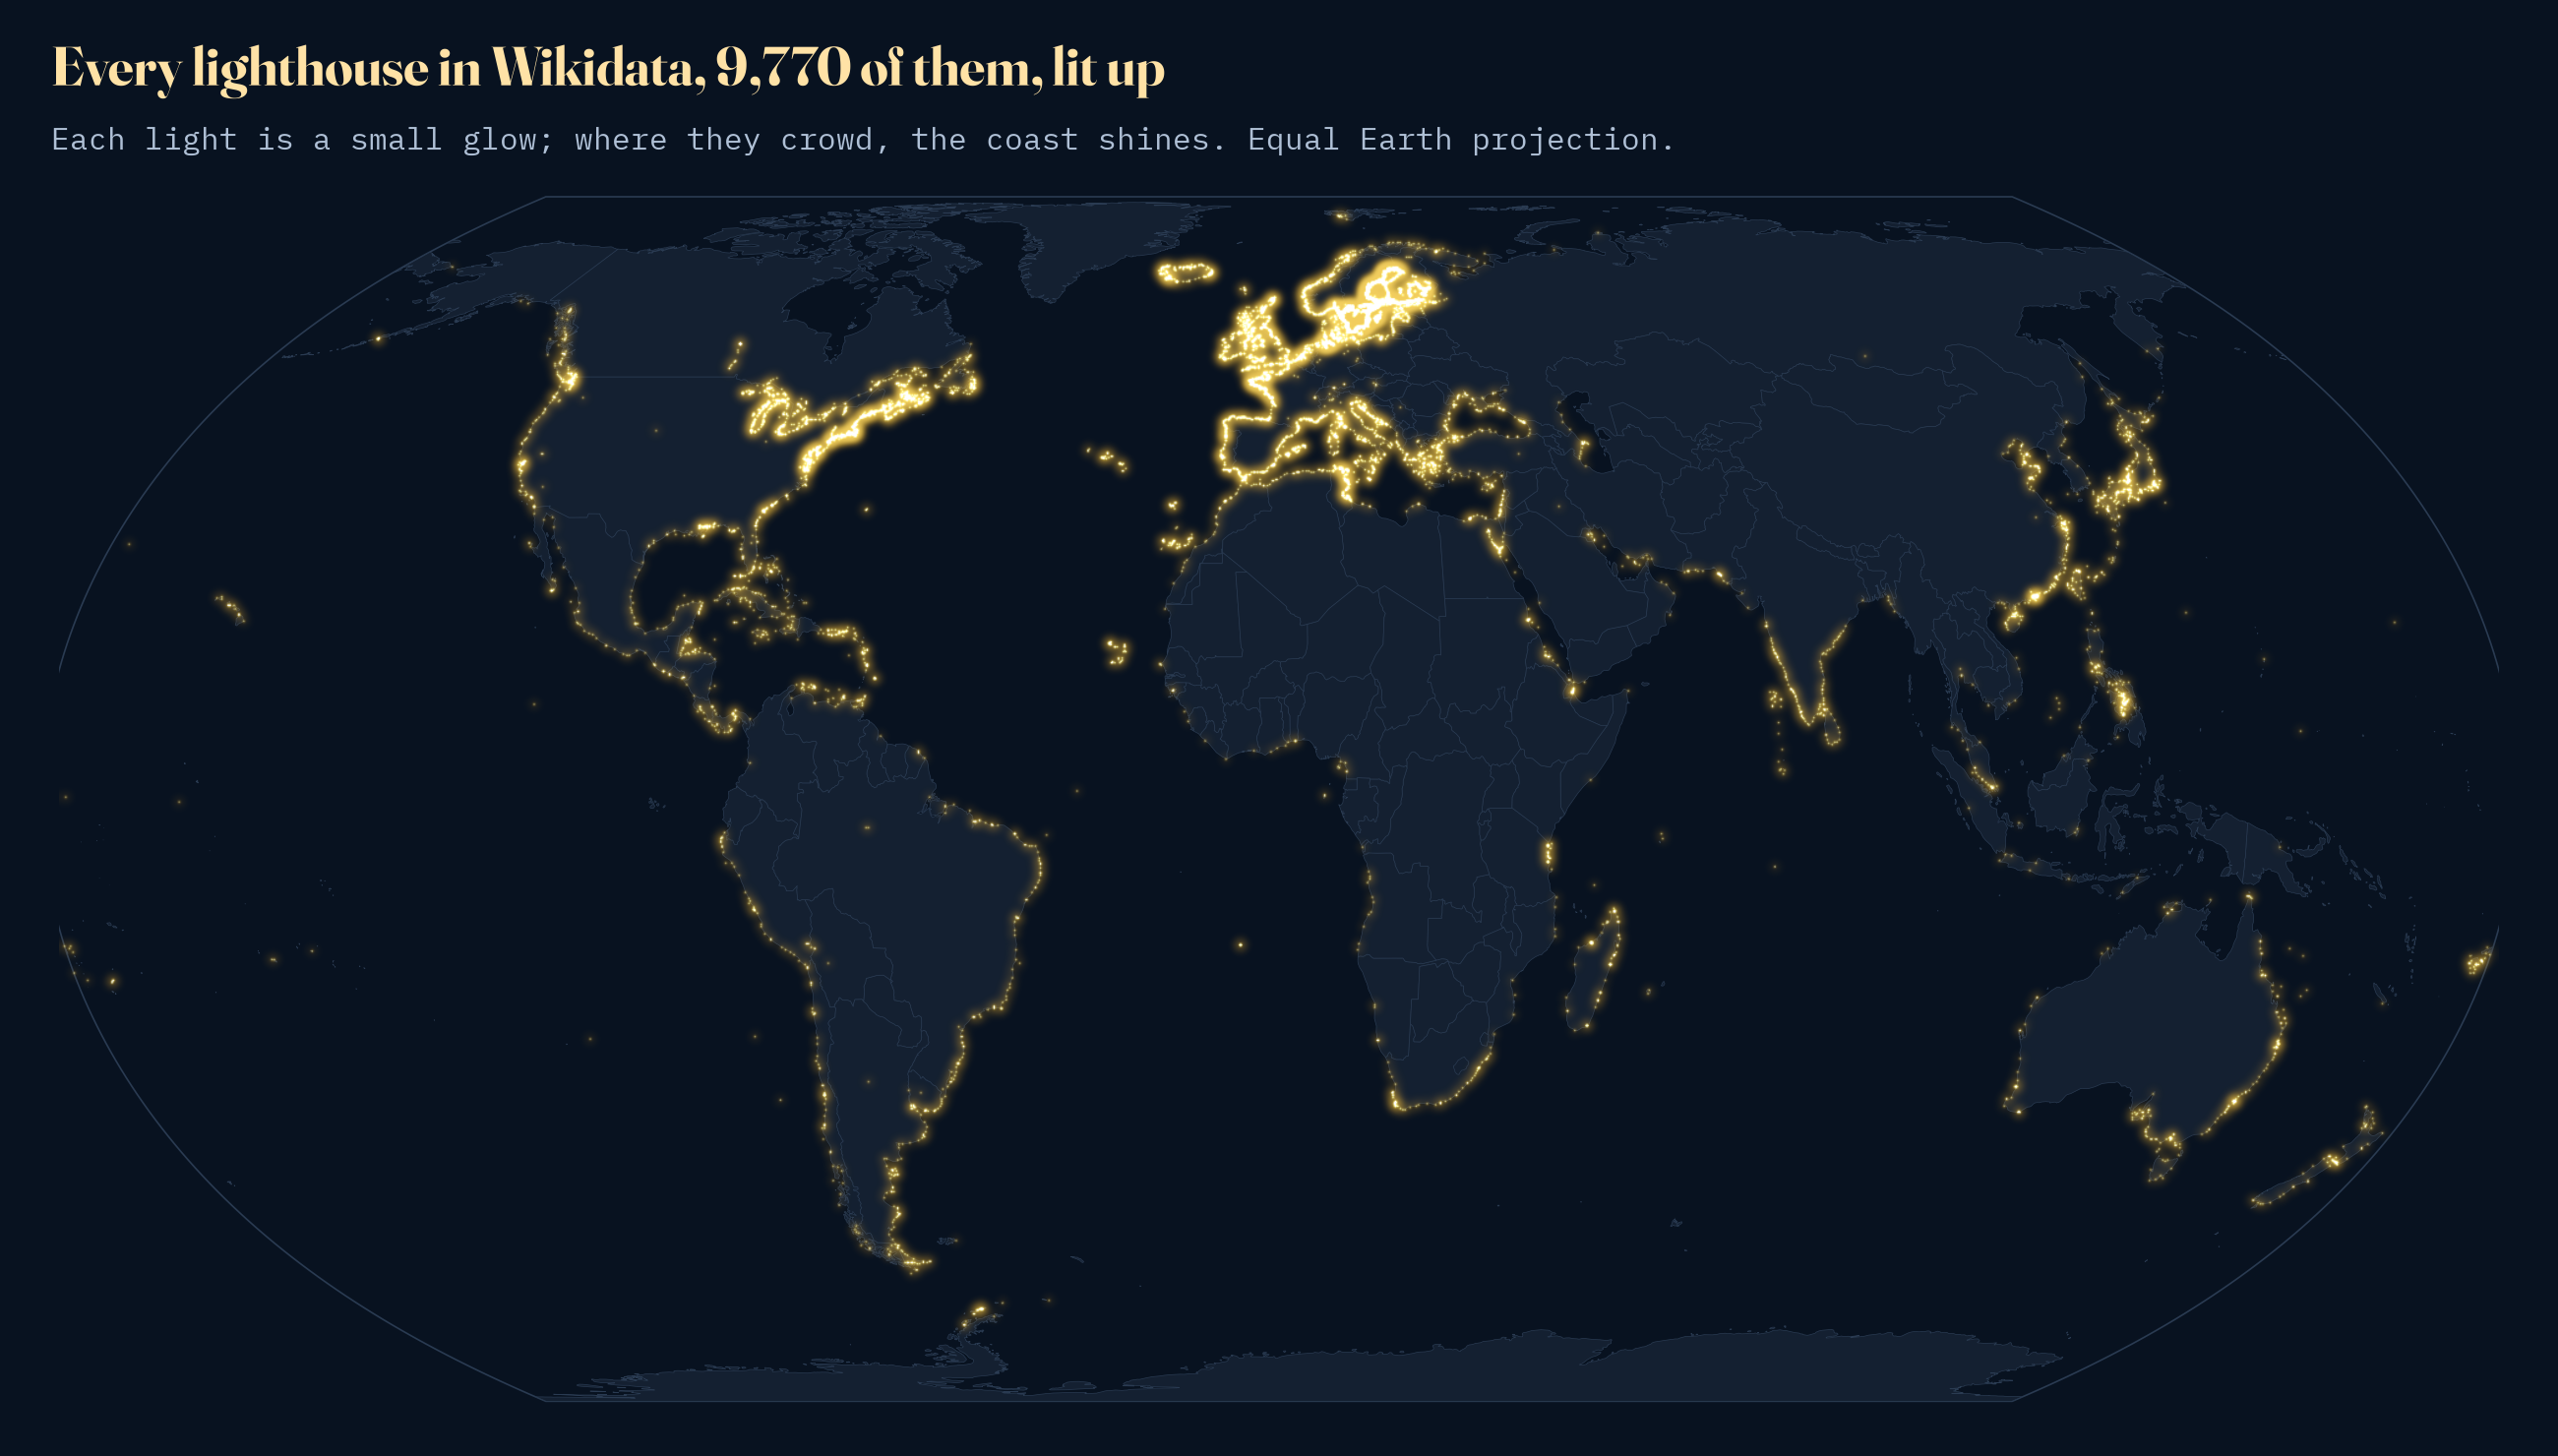
\includegraphics[width=\textwidth]{f_glow_world.png}
\caption{Every lighthouse in Wikidata, drawn as a glow on a night map (Equal Earth projection).}\label{fig:glow}\end{figure}

\begin{figure}[tbp]\centering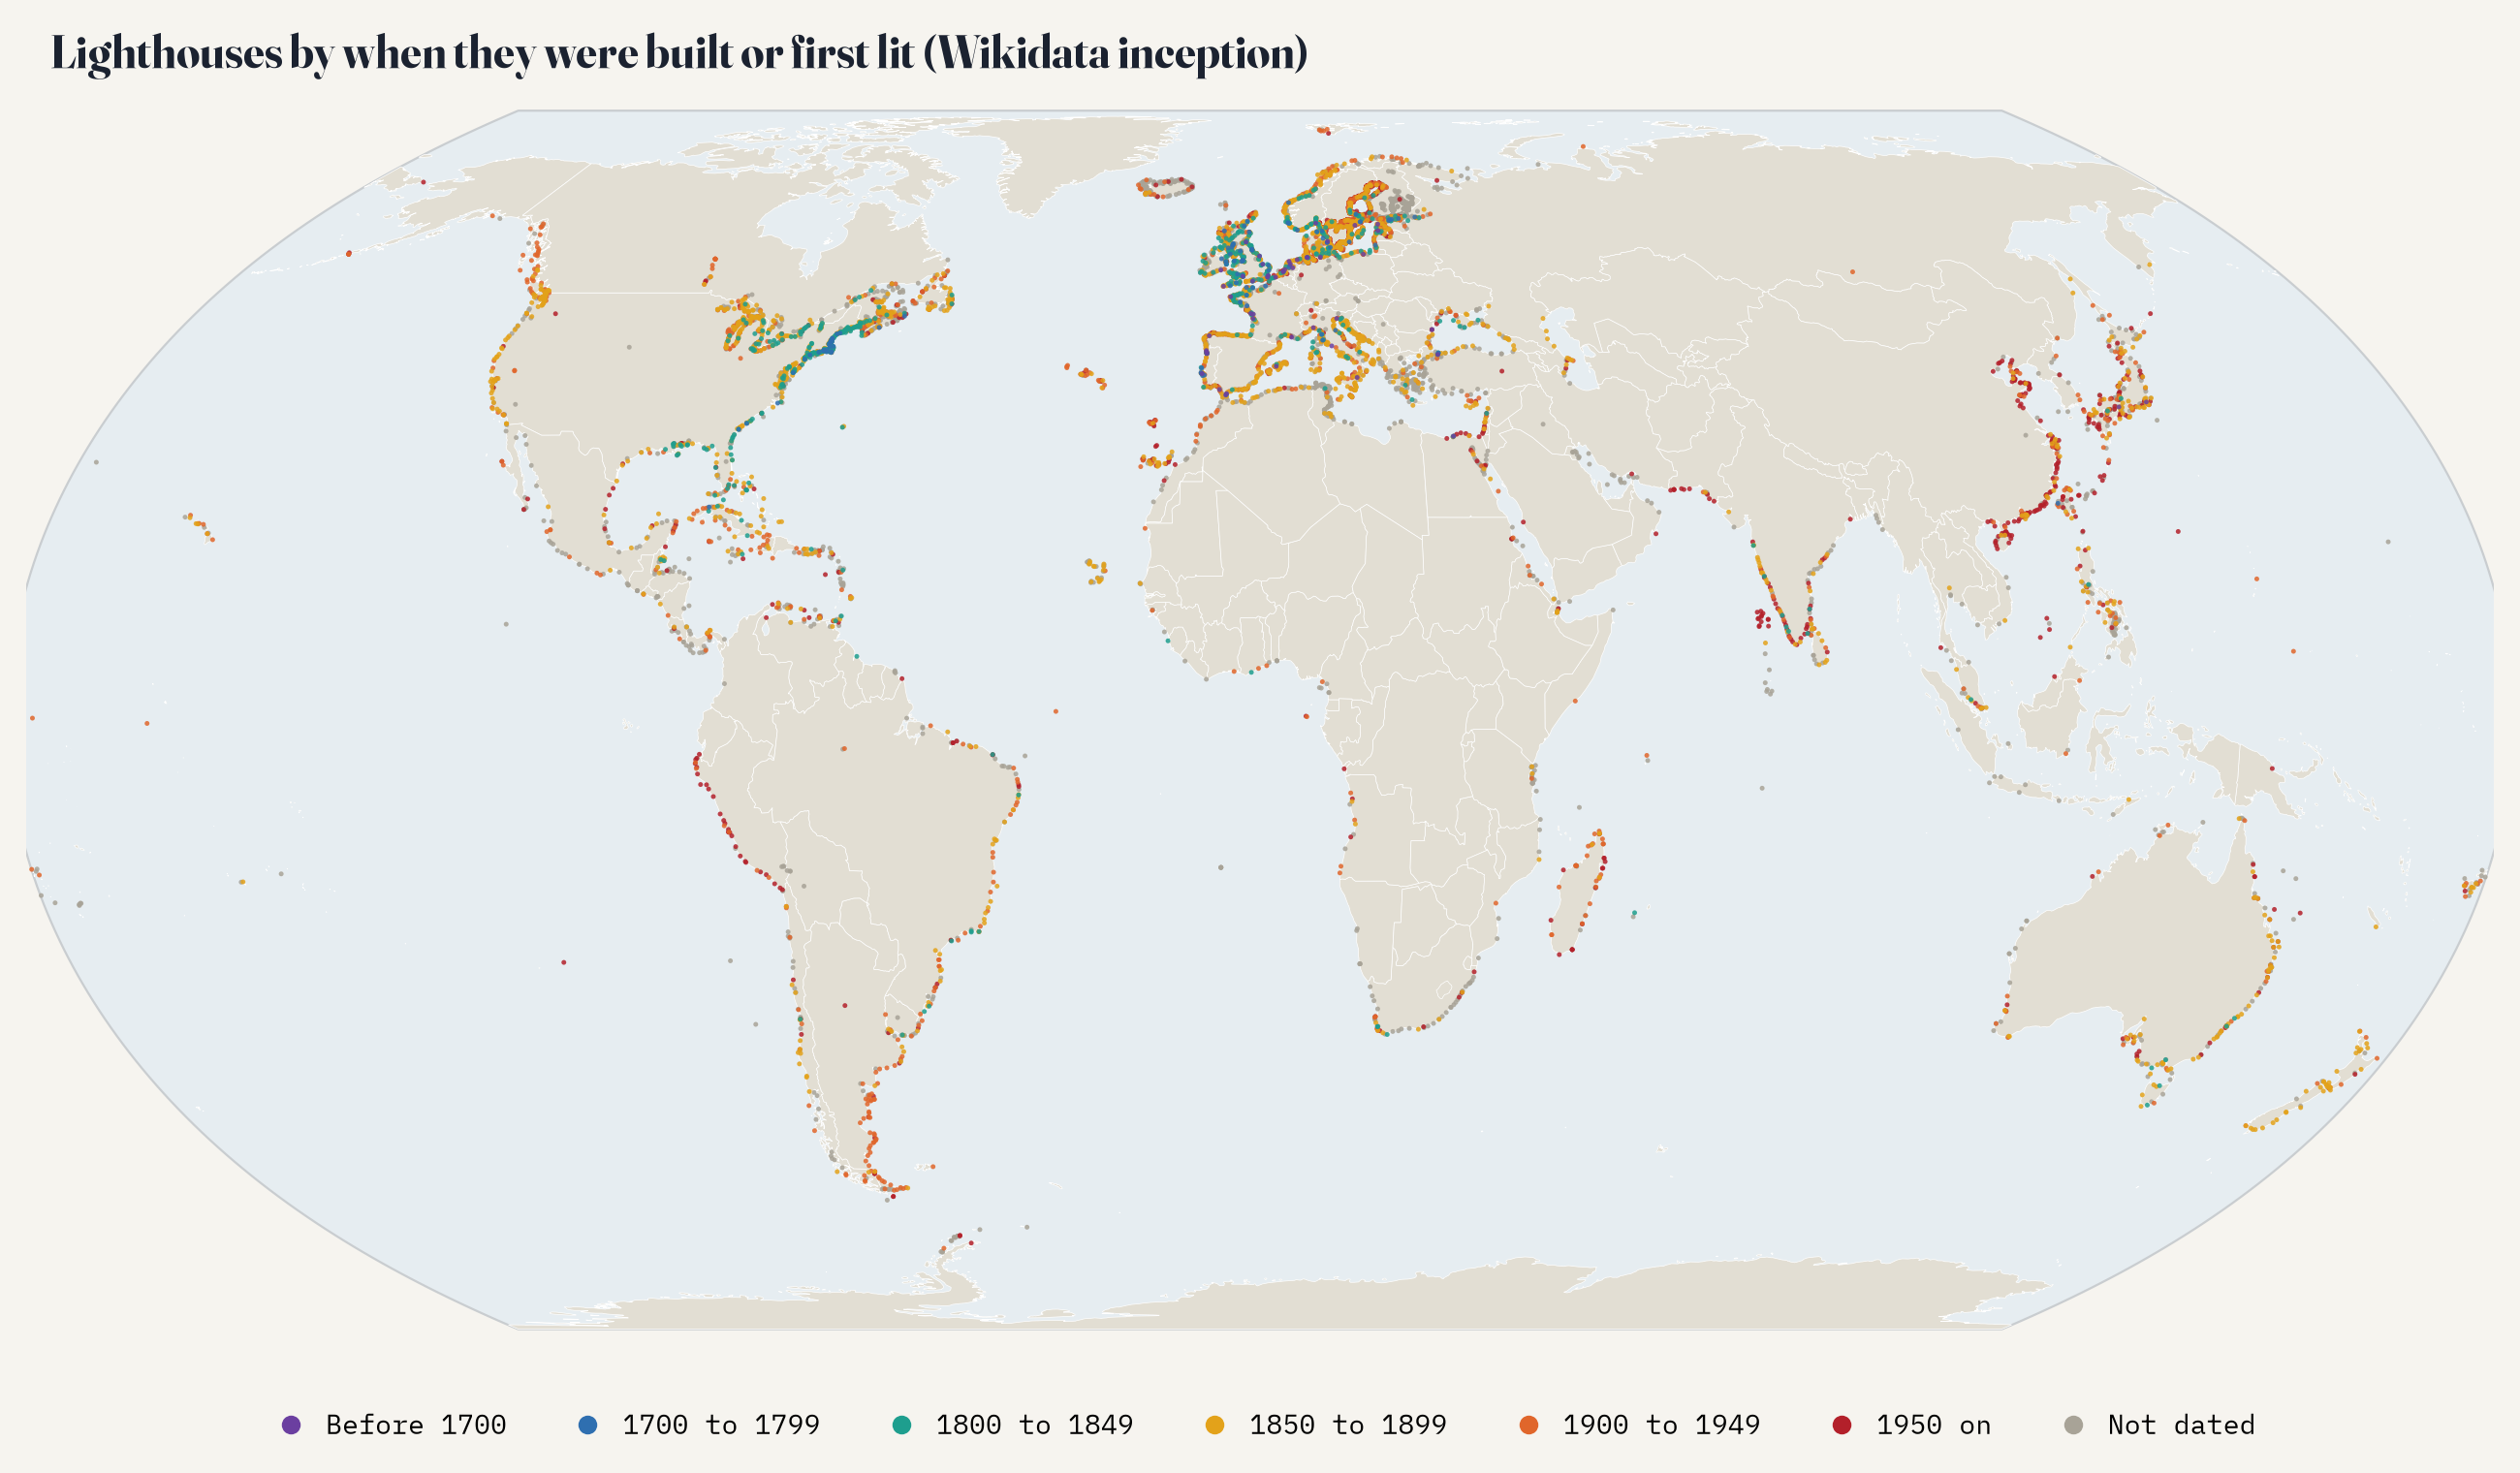
\includegraphics[width=\textwidth]{f_era_map.png}
\caption{Lighthouses by the period of their earliest Wikidata inception date.}\label{fig:era}\end{figure}

\begin{table}[tbp]\centering\small\caption{The twenty countries with most lighthouses in Wikidata. Inland: lake and river lights. Coast: Natural Earth 1:10m. Bare: share with at most one Wikipedia article.}\label{tab:countries}\begin{tabular}{lrrrrr}\toprule Country & Lights & Inland & Coast km & Sea lights per 1,000 km & Bare\\\midrule
Sweden & 2,555 & 327 & 6,541 & 340.6 & 96\%\\
United States & 923 & 284 & 68,168 & 9.4 & 16\%\\
Finland & 794 & 267 & 4,199 & 125.5 & 91\%\\
Canada & 473 & 74 & 137,270 & 2.9 & 67\%\\
United Kingdom & 468 & 6 & 11,855 & 39.0 & 38\%\\
France & 307 & 3 & 6,284 & 48.4 & 27\%\\
Japan & 238 & 2 & 15,474 & 15.3 & 54\%\\
Spain & 234 & 0 & 5,000 & 46.8 & 9\%\\
Germany & 225 & 35 & 2,663 & 71.4 & 41\%\\
Italy & 221 & 11 & 6,022 & 34.9 & 20\%\\
Norway & 216 & 0 & 27,511 & 7.9 & 21\%\\
Australia & 175 & 1 & 33,866 & 5.1 & 21\%\\
China & 153 & 1 & 16,352 & 9.3 & 90\%\\
Iceland & 122 & 0 & 5,213 & 23.4 & 50\%\\
Tunisia & 118 & 0 & 1,387 & 85.1 & 83\%\\
Greece & 111 & 0 & 9,480 & 11.7 & 73\%\\
Brazil & 105 & 5 & 18,674 & 5.4 & 31\%\\
Portugal & 104 & 0 & 2,120 & 49.1 & 15\%\\
India & 102 & 0 & 11,014 & 9.3 & 71\%\\
Russia & 100 & 6 & 76,557 & 1.2 & 37\%\\
\bottomrule\end{tabular}\end{table}

\begin{figure}[tbp]\centering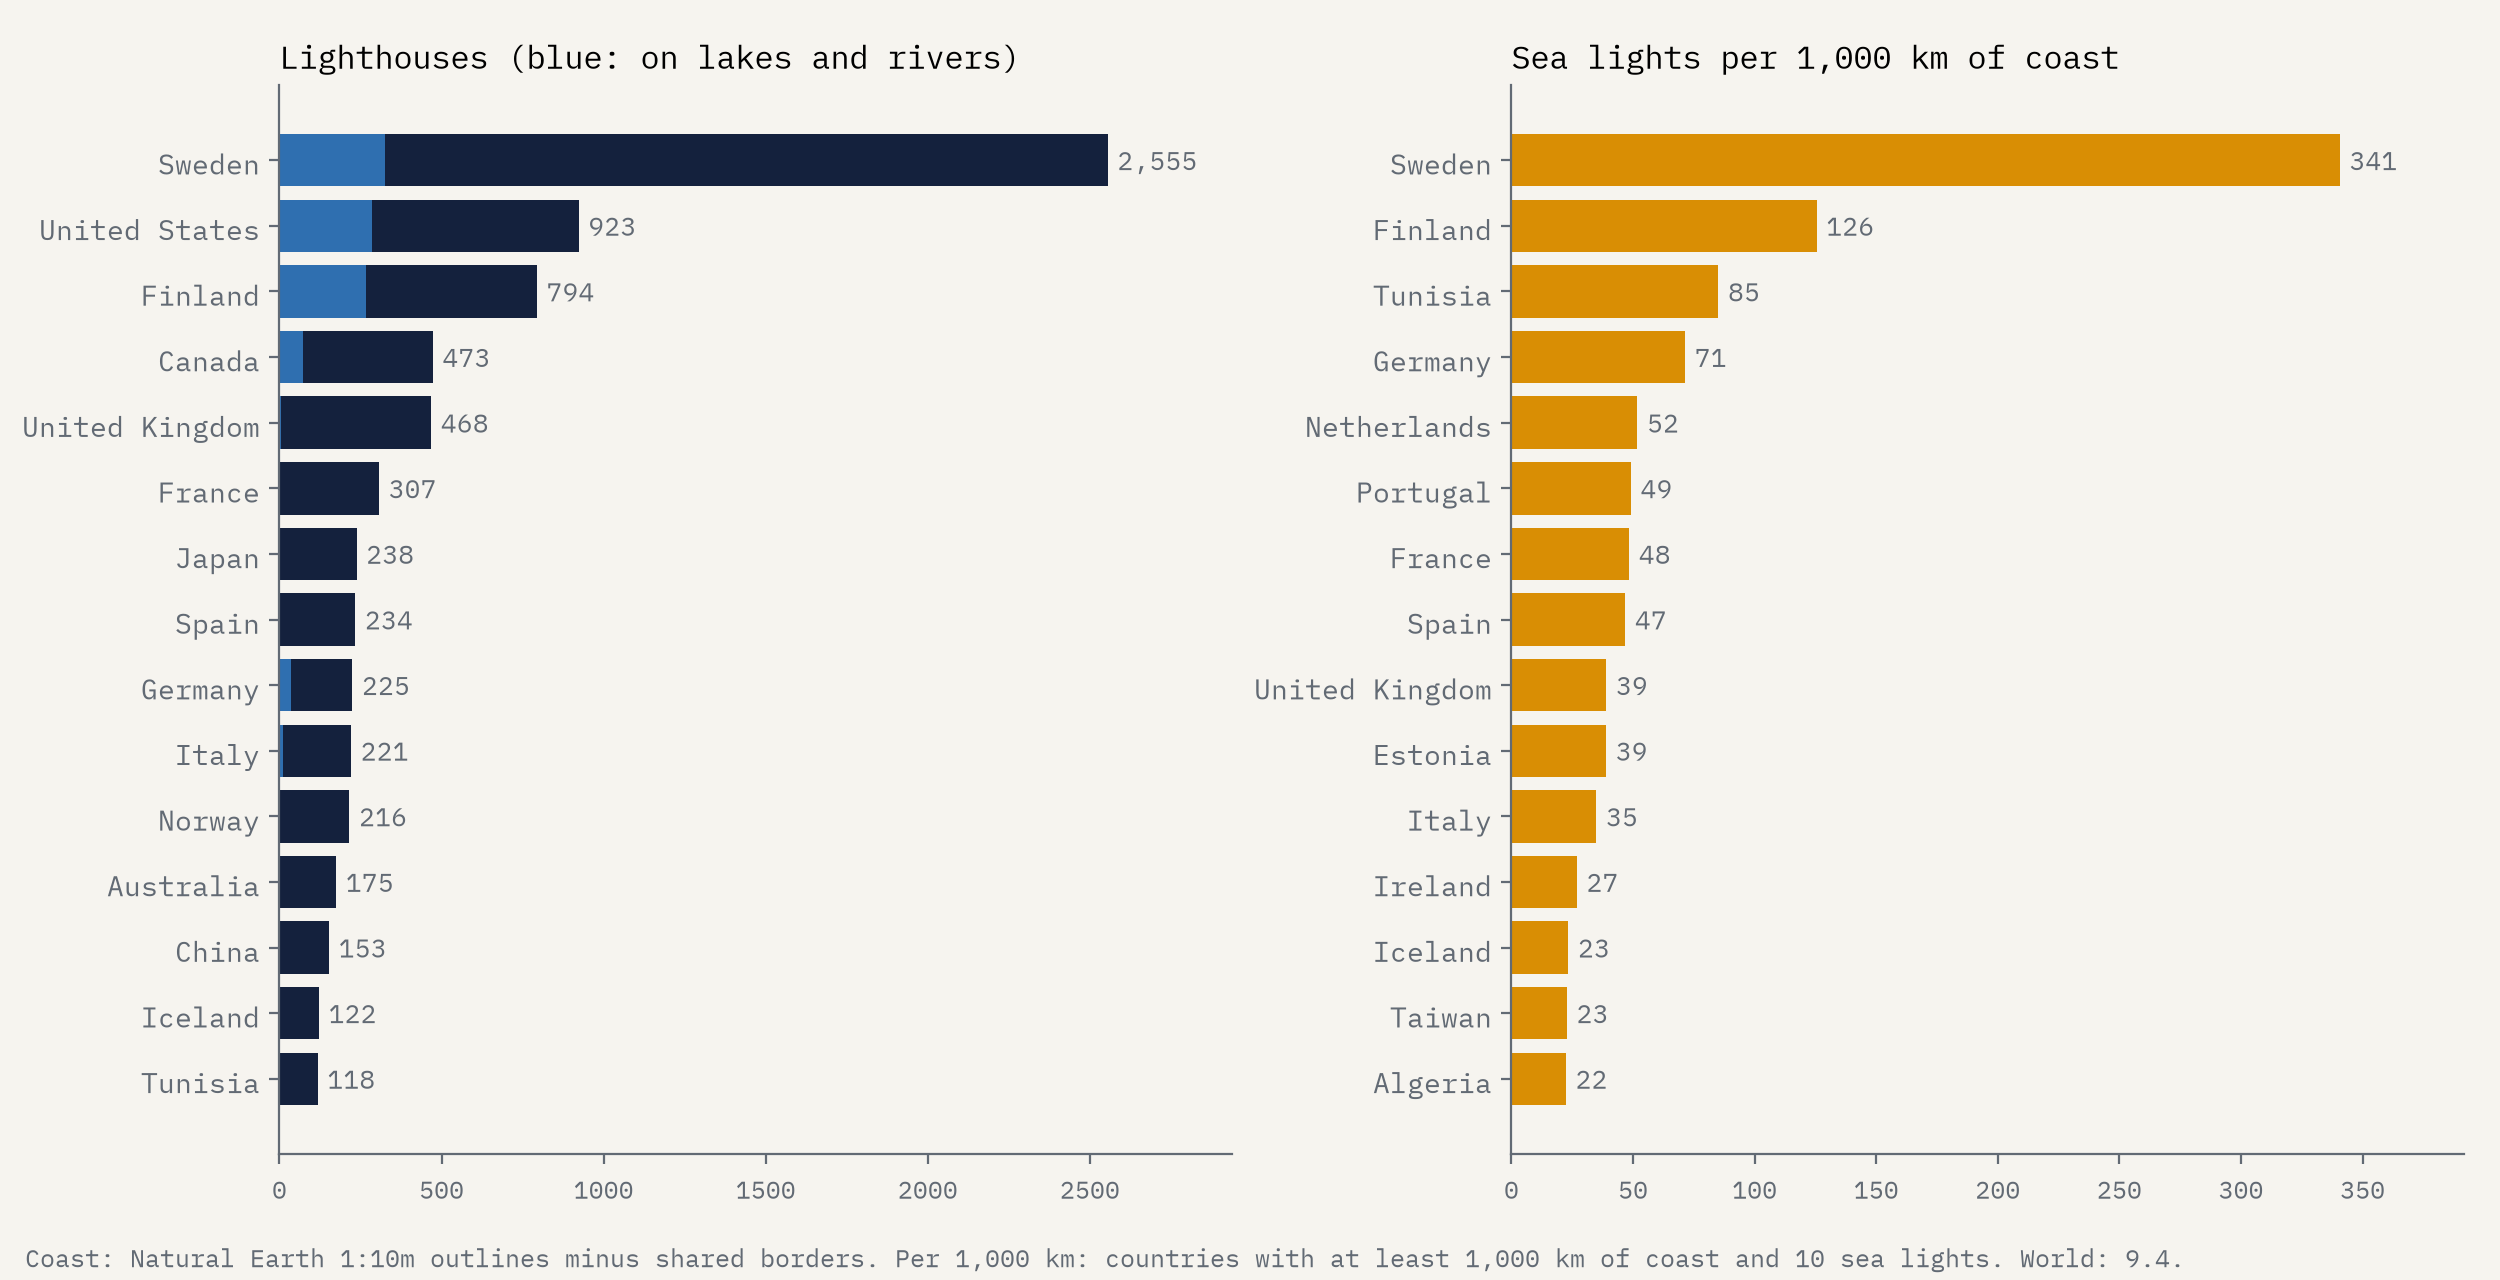
\includegraphics[width=\textwidth]{f_countries.png}
\caption{Lighthouses by country (left; blue: lake and river lights) and sea lights per 1,000~km of coast (right).}\label{fig:countries}\end{figure}

The densest regional coasts (Table~\ref{tab:regions}, Figure~\ref{fig:regions}) are all in Sweden and Finland: Västra Götaland, on the Skagerrak, has 71.9 sea lights per 100~km, Blekinge 66.9 and Skåne 56.5. Outside Sweden and Finland the densest are Lower Saxony (13.8), on the Wadden Sea, Connecticut (12.9), on Long Island Sound, and Bizerte in Tunisia (11.7). Figure~\ref{fig:north} shows northern Europe at night.

\begin{table}[tbp]\centering\small\caption{The densest regional coasts: sea lights per 100~km, regions with at least 150 km of coast and 15 sea lights.}\label{tab:regions}\begin{tabular}{llrrr}\toprule Region & Country & Sea lights & Coast km & Per 100 km\\\midrule
Västra Götaland & Sweden & 407 & 566 & 71.9\\
Blekinge & Sweden & 139 & 208 & 66.9\\
Skåne & Sweden & 222 & 393 & 56.5\\
Halland & Sweden & 80 & 209 & 38.3\\
Gävleborg & Sweden & 127 & 370 & 34.4\\
Stockholm & Sweden & 345 & 1,069 & 32.3\\
Östergötland & Sweden & 103 & 343 & 30.0\\
Kalmar & Sweden & 196 & 701 & 28.0\\
Uppsala & Sweden & 56 & 253 & 22.1\\
Uusimaa & Finland & 146 & 685 & 21.3\\
Norrbotten & Sweden & 146 & 686 & 21.3\\
Västerbotten & Sweden & 114 & 542 & 21.0\\
Gotland & Sweden & 91 & 460 & 19.8\\
Kymenlaakso & Finland & 43 & 238 & 18.0\\
Västernorrland & Sweden & 97 & 598 & 16.2\\
Lower Saxony & Germany & 82 & 593 & 13.8\\
Connecticut & United States & 28 & 216 & 12.9\\
Bizerte & Tunisia & 23 & 197 & 11.7\\
Finistère & France & 65 & 592 & 11.0\\
Livorno & Italy & 26 & 239 & 10.9\\
\bottomrule\end{tabular}\end{table}

\begin{figure}[tbp]\centering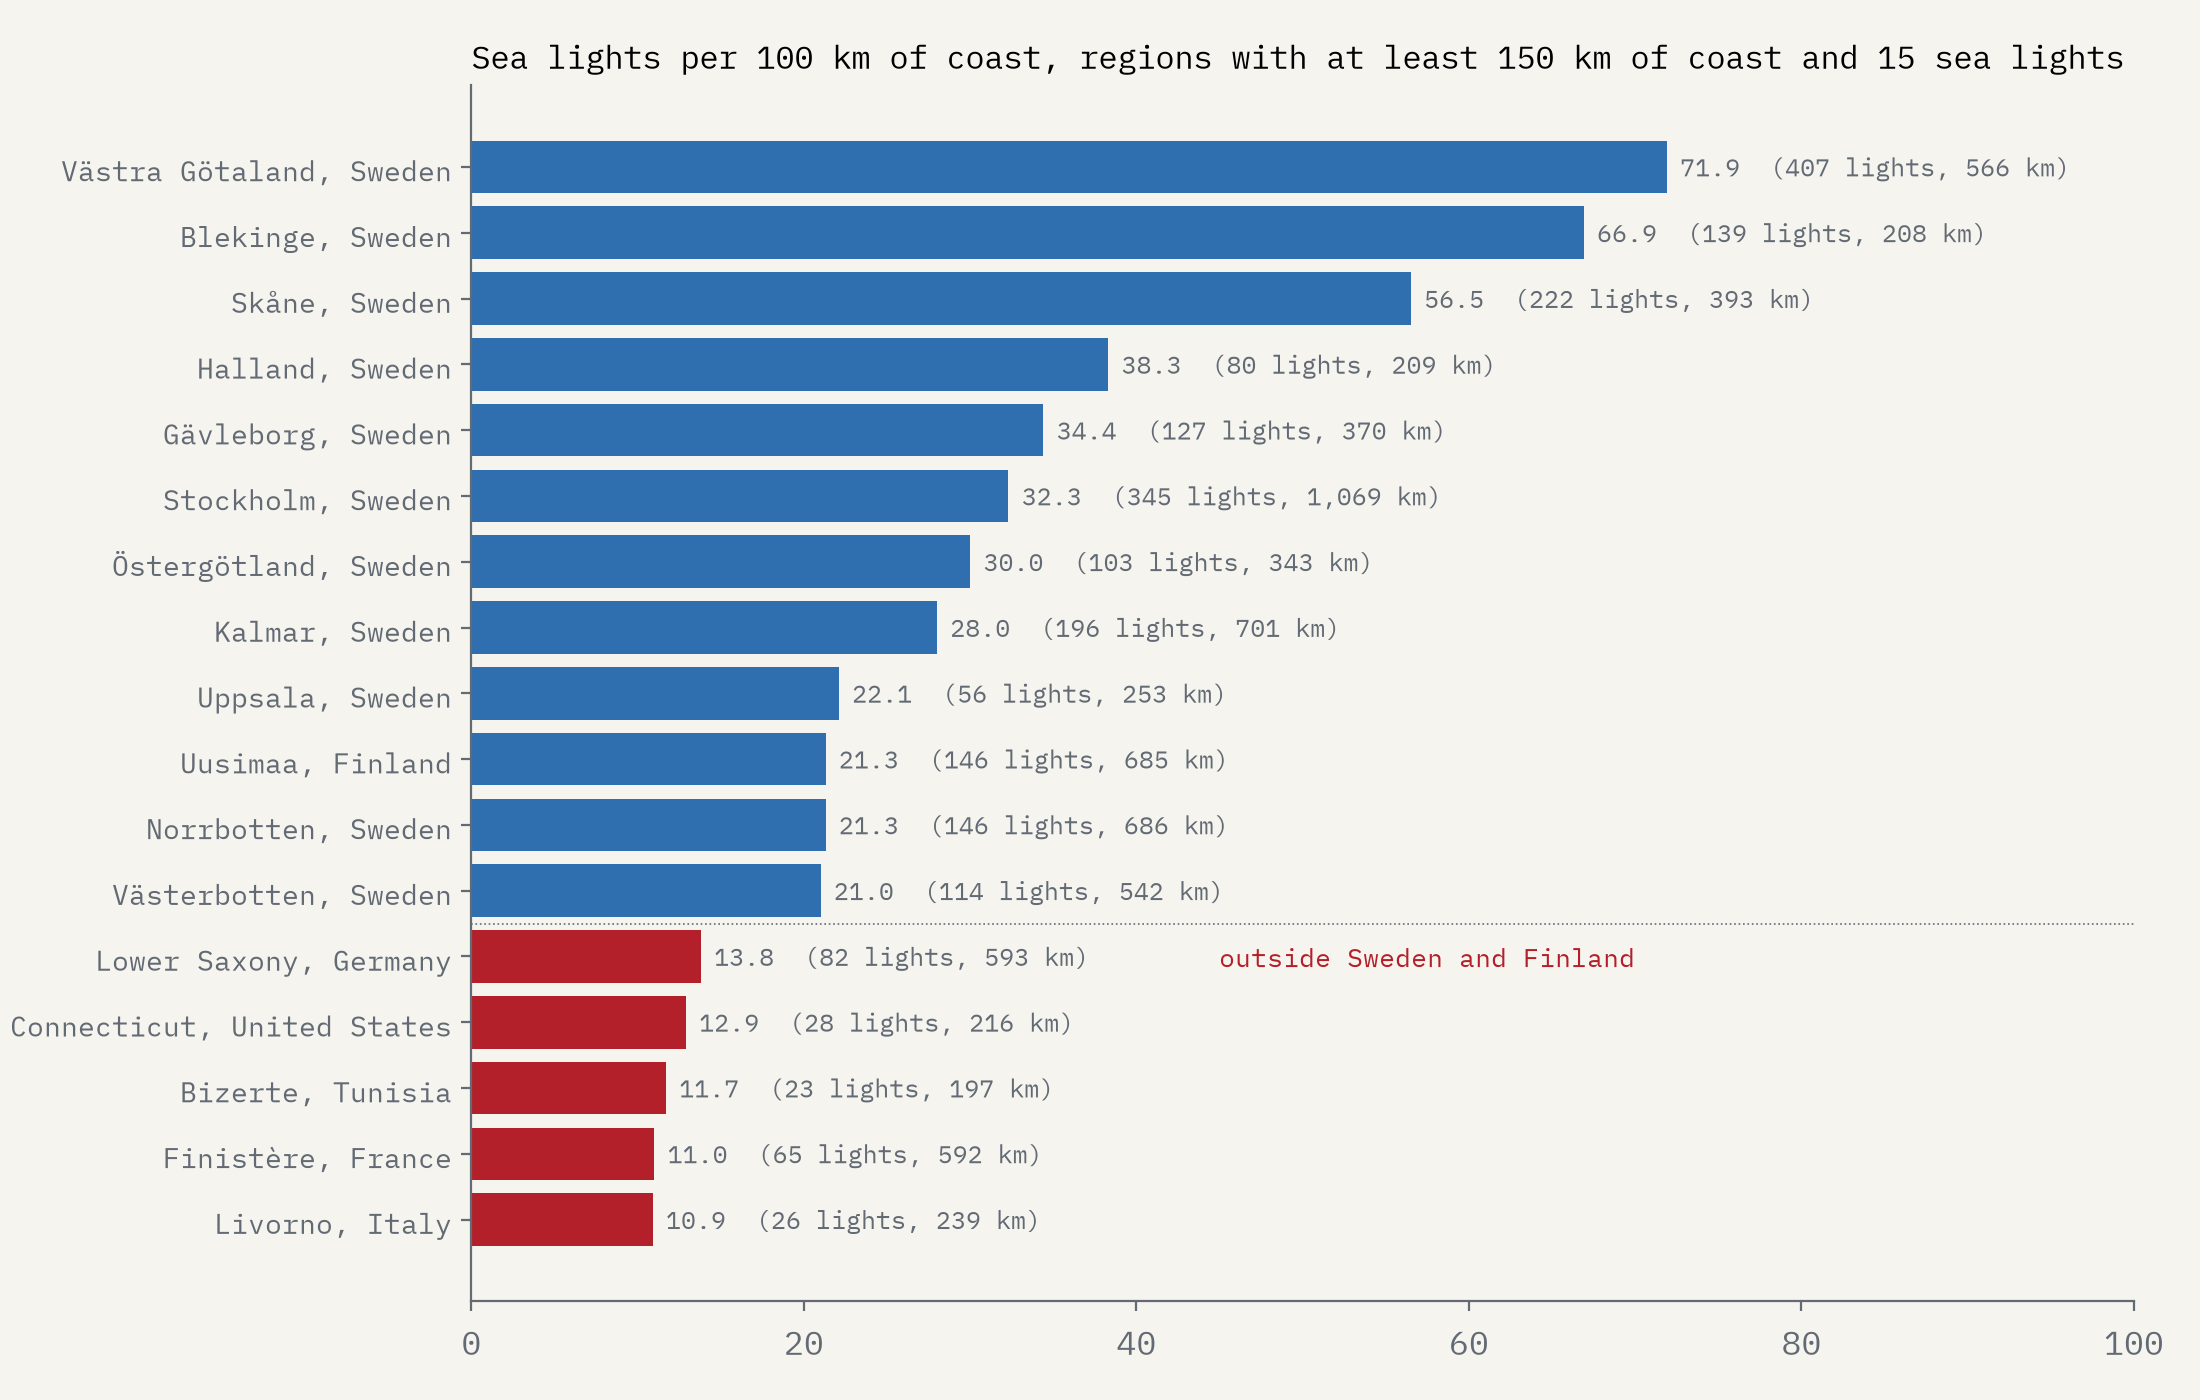
\includegraphics[width=.92\textwidth]{f_regions.png}
\caption{Sea lights per 100~km of coast for regions with at least 150 km of coast and 15 sea lights: the twelve densest, and the densest outside Sweden and Finland.}\label{fig:regions}\end{figure}

\begin{figure}[tbp]\centering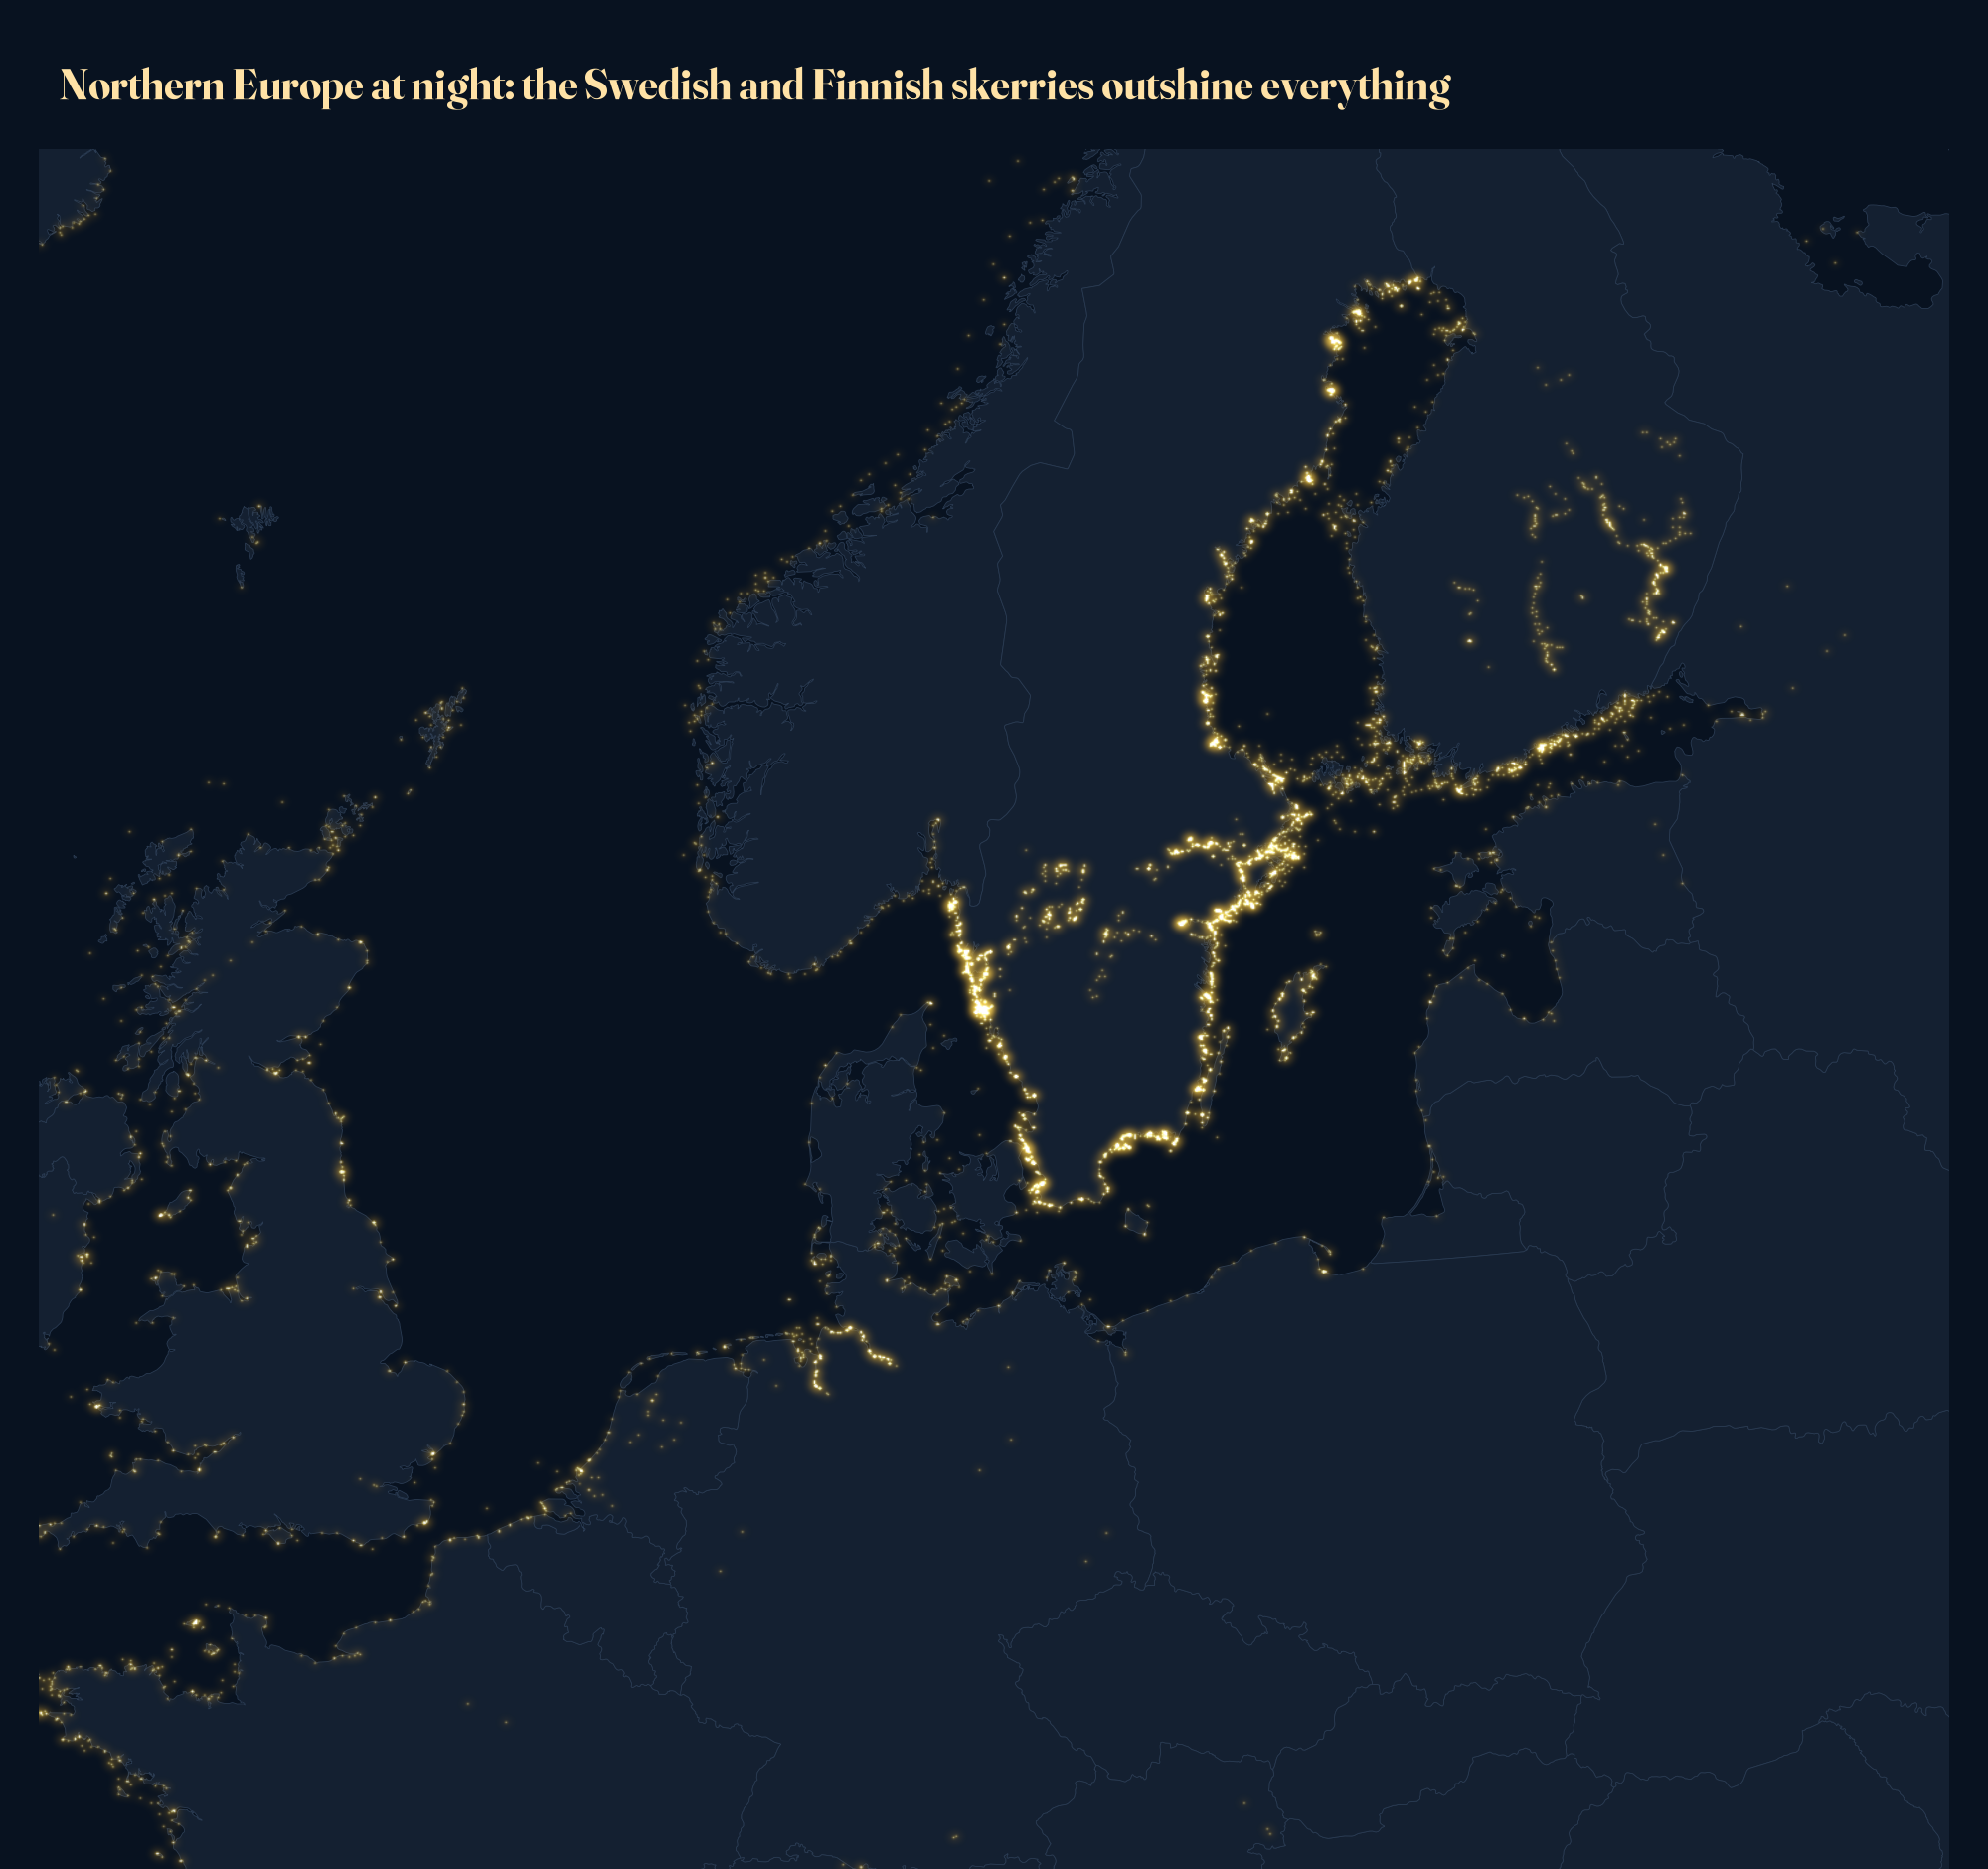
\includegraphics[width=.8\textwidth]{f_glow_north.png}
\caption{Northern Europe at night, one glow per lighthouse.}\label{fig:north}\end{figure}

\subsection{When}
Of the 6,546 dated lights, 17 are dated before 1500 and 144 before 1800 (Figure~\ref{fig:timeline}). Outside Sweden, new lights rise from 103 in the 1820s to 376 in the 1870s and remain above 300 a decade until the 1910s; the United States peaks in the 1870s (96). The average falls from 337 a decade in 1850 to 1909 to 97 in 1970 to 2019, a factor of 3.5. Sweden's lights follow a different curve, peaking in the 1940s with 326; from 1930 to 1969 Sweden supplies 70\% of all dated new lights. The Swedish lights of 1930 to 1969 are small (median recorded height 8.9 for 227 with a height, against 16.0 for 1,468 lights built elsewhere in 1850 to 1909; most heights are in metres) and 89\% have no Wikipedia article. With all countries together, the busiest decade is the 1900s (500).

\begin{figure}[tbp]\centering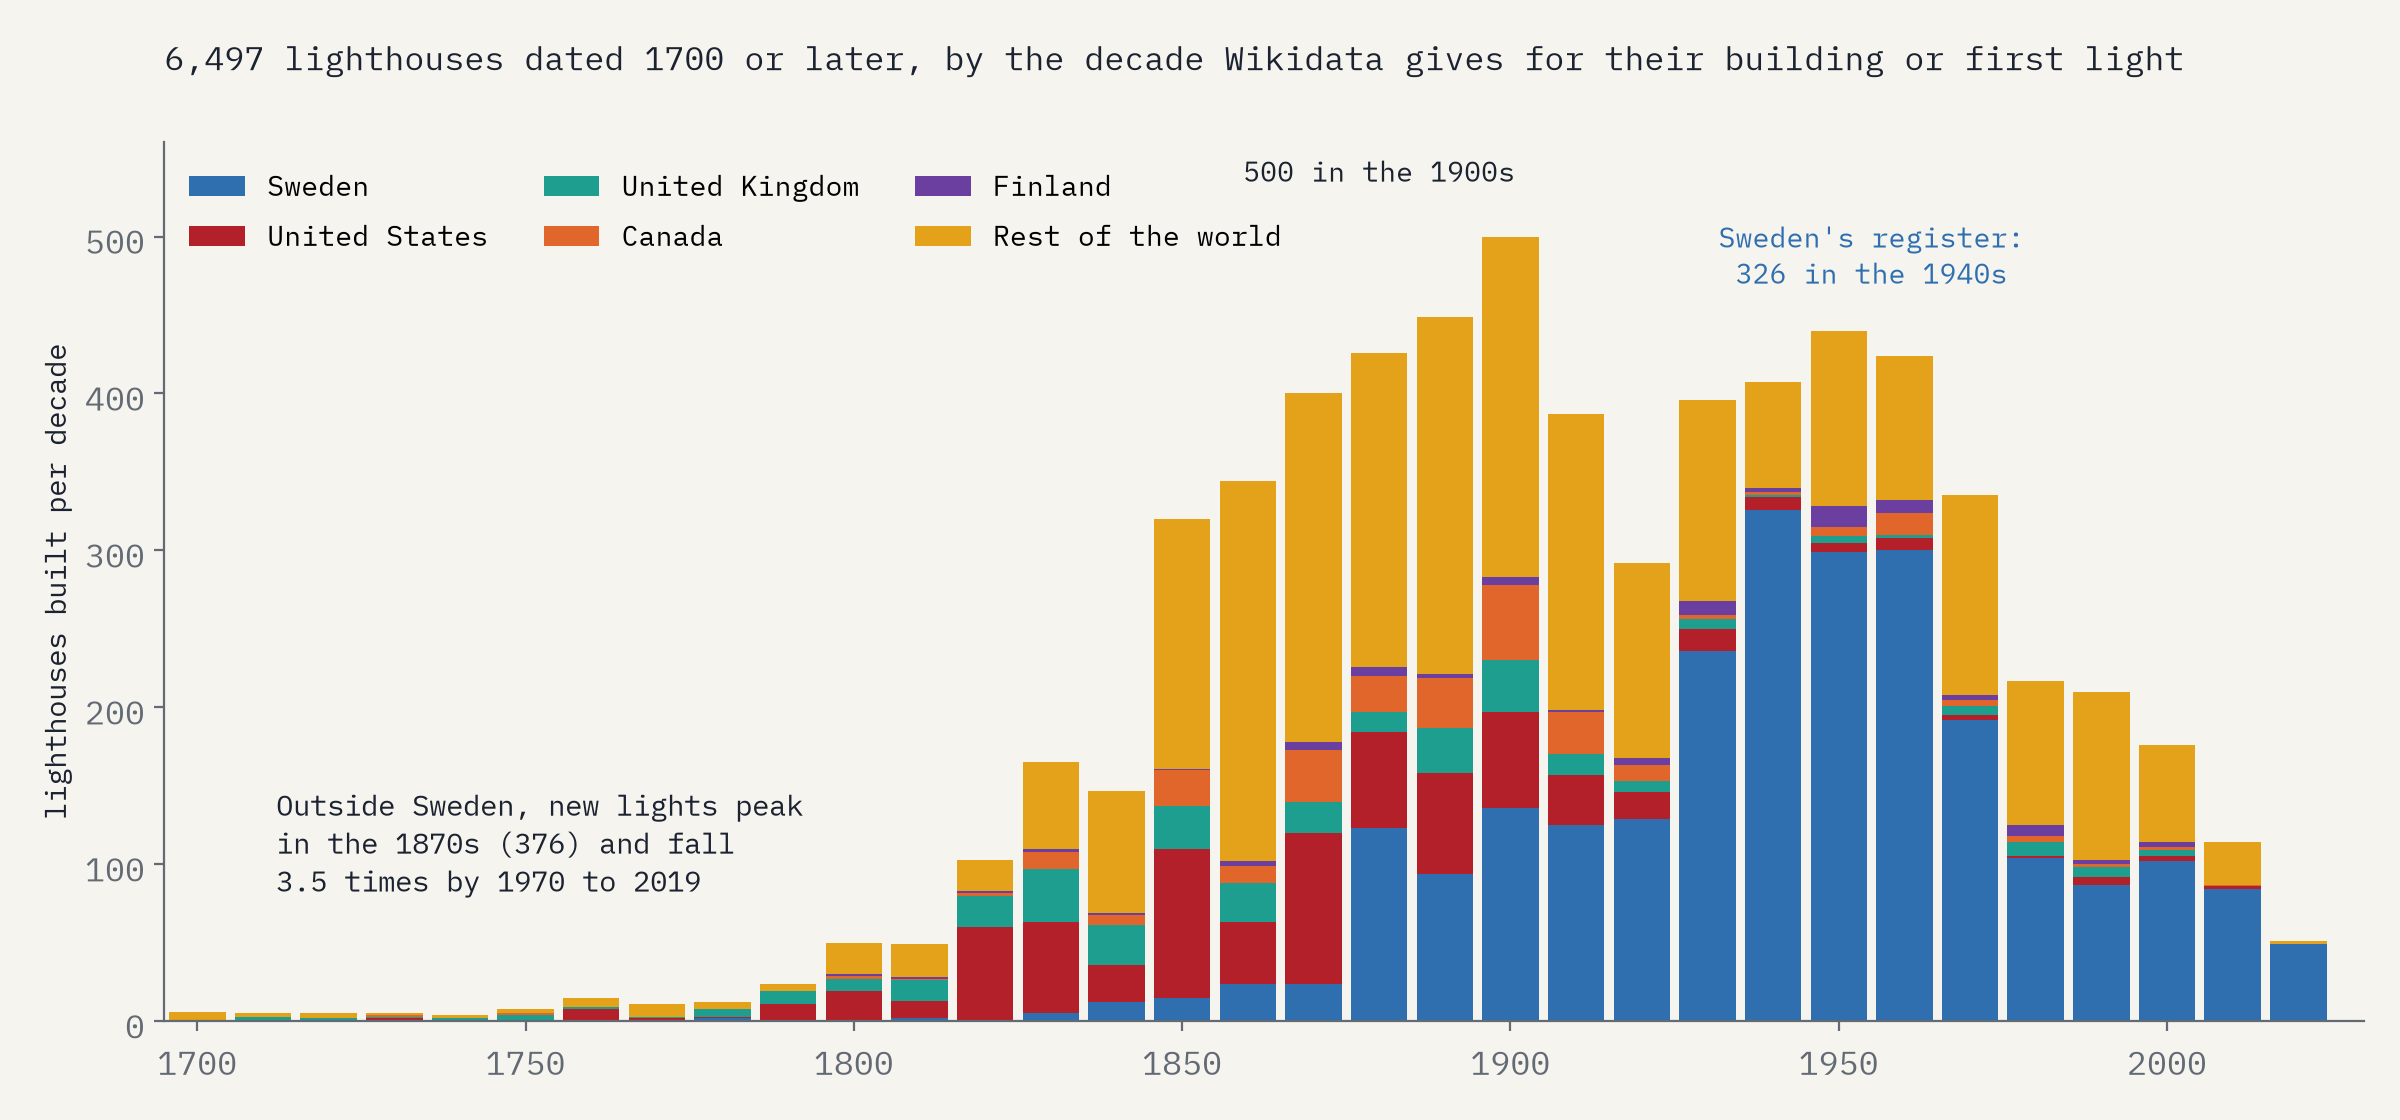
\includegraphics[width=\textwidth]{f_timeline.png}
\caption{Lighthouses built per decade, by the earliest Wikidata inception year, by country.}\label{fig:timeline}\end{figure}

\subsection{The oldest}
Table~\ref{tab:oldest} lists the oldest dated lights. The two oldest dates belong to lost towers, the Lighthouse of Alexandria (278~BC) and the Tower of Caepio. The oldest still standing is the Tower of Hercules at A Coruña (AD~100), followed by the Roman Dubris Pharos at Dover (AD~200) and medieval towers such as Hook Head (dated 1300 in Wikidata, apparently rounded to a century). Several old dates belong to sites rather than towers: the Planier light is dated 1326 in Wikidata but its present tower is from 1959 according to the Wikipedia list.

\begin{table}[tbp]\centering\footnotesize\caption{The oldest dated lighthouses in Wikidata (inception year), with their status today where checked by hand.}\label{tab:oldest}\begin{tabular}{rp{3.8cm}p{2.4cm}lp{5.0cm}}\toprule Year & Lighthouse & Country & Today & Note\\\midrule
278~BC & Lighthouse of Alexandria & Egypt & Lost & Fell to earthquakes in the Middle Ages; nothing stands\\
139~BC & Tower of Caepio & Spain & Lost & Known from ancient writers; the tower is gone\\
AD~100 & Tower of Hercules & Spain & Standing & Roman tower, refaced in the 1700s; still lit\\
AD~200 & Dubris Pharos & United Kingdom & Standing & Roman tower inside Dover Castle, a ruin\\
1110 & Maiden's Tower & Turkey & Rebuilt & Tower on the islet rebuilt several times since\\
1200 & Caorle Lighthouse & Italy & Not checked & \\
1284 & Grote Vierboete & Belgium & Not checked & \\
1300 & Hook Lighthouse & Ireland & Standing & Medieval tower, still lit; the year is Wikidata's and looks rounded to a century\\
1300 & Portopí Lighthouse & Spain & Standing & Still lit, at the port of Palma\\
1300 & Genoese Lighthouse & Romania & Rebuilt & Wikidata's date is the Genoese era it commemorates; the tower is from 1860\\
1310 & Great Tower Neuwerk & Germany & Standing & Medieval tower on Neuwerk island\\
1326 & Planier Light & France & Rebuilt & The present tower is from 1959 (Wikipedia list of tallest lighthouses)\\
1328 & St Catherine's Oratory & United Kingdom & Standing & Medieval oratory tower on St Catherine's Down, Isle of Wight\\
1350 & St Andrew's Church & United Kingdom & Not checked & \\
1350 & Lighthouse of Oostvoorne & Netherlands & Not checked & \\
1468 & Tour de la Lanterne & France & Standing & Tower at the harbour of La Rochelle\\
1482 & Wisłoujście Fortress & Poland & Standing & Fortress tower at the mouth of the Vistula, Gdańsk\\
1527 & São Miguel-o-Anjo Lighthouse & Portugal & Not checked & \\
1531 & Kõpu Lighthouse & Estonia & Standing & Still lit, on Hiiumaa\\
1539 & Leuchtturm Travemünde & Germany & Standing & Old tower, now a museum\\
1543 & Lighthouse of Genoa & Italy & Standing & Rebuilt in 1543 and still lit (Wikipedia list of tallest lighthouses)\\
1555 & Punta San Raineri Lighthouse & Italy & Not checked & \\
1563 & No English label (Q108542562) & Sweden & Not checked & \\
1576 & Old Lighthouse Borkum & Germany & Not checked & \\
\bottomrule\end{tabular}\end{table}

\subsection{The tallest}
The 28 towers in the Wikipedia list (Figure~\ref{fig:tallest}) range from 60~m to the 83~m of the Île Vierge lighthouse (1902). 16 are stone, granite or brick, and 11 were built before 1900. I matched 26 of them to Wikidata items in the same country: 19 have a Wikidata height within 3~m of the list's metres, 1 (Cape Hatteras, 210) matches the height in feet, 2 differs and 6 have none. Wikidata gives a height for 4,066 lights in all; without units these cannot be ranked safely.

\begin{figure}[tbp]\centering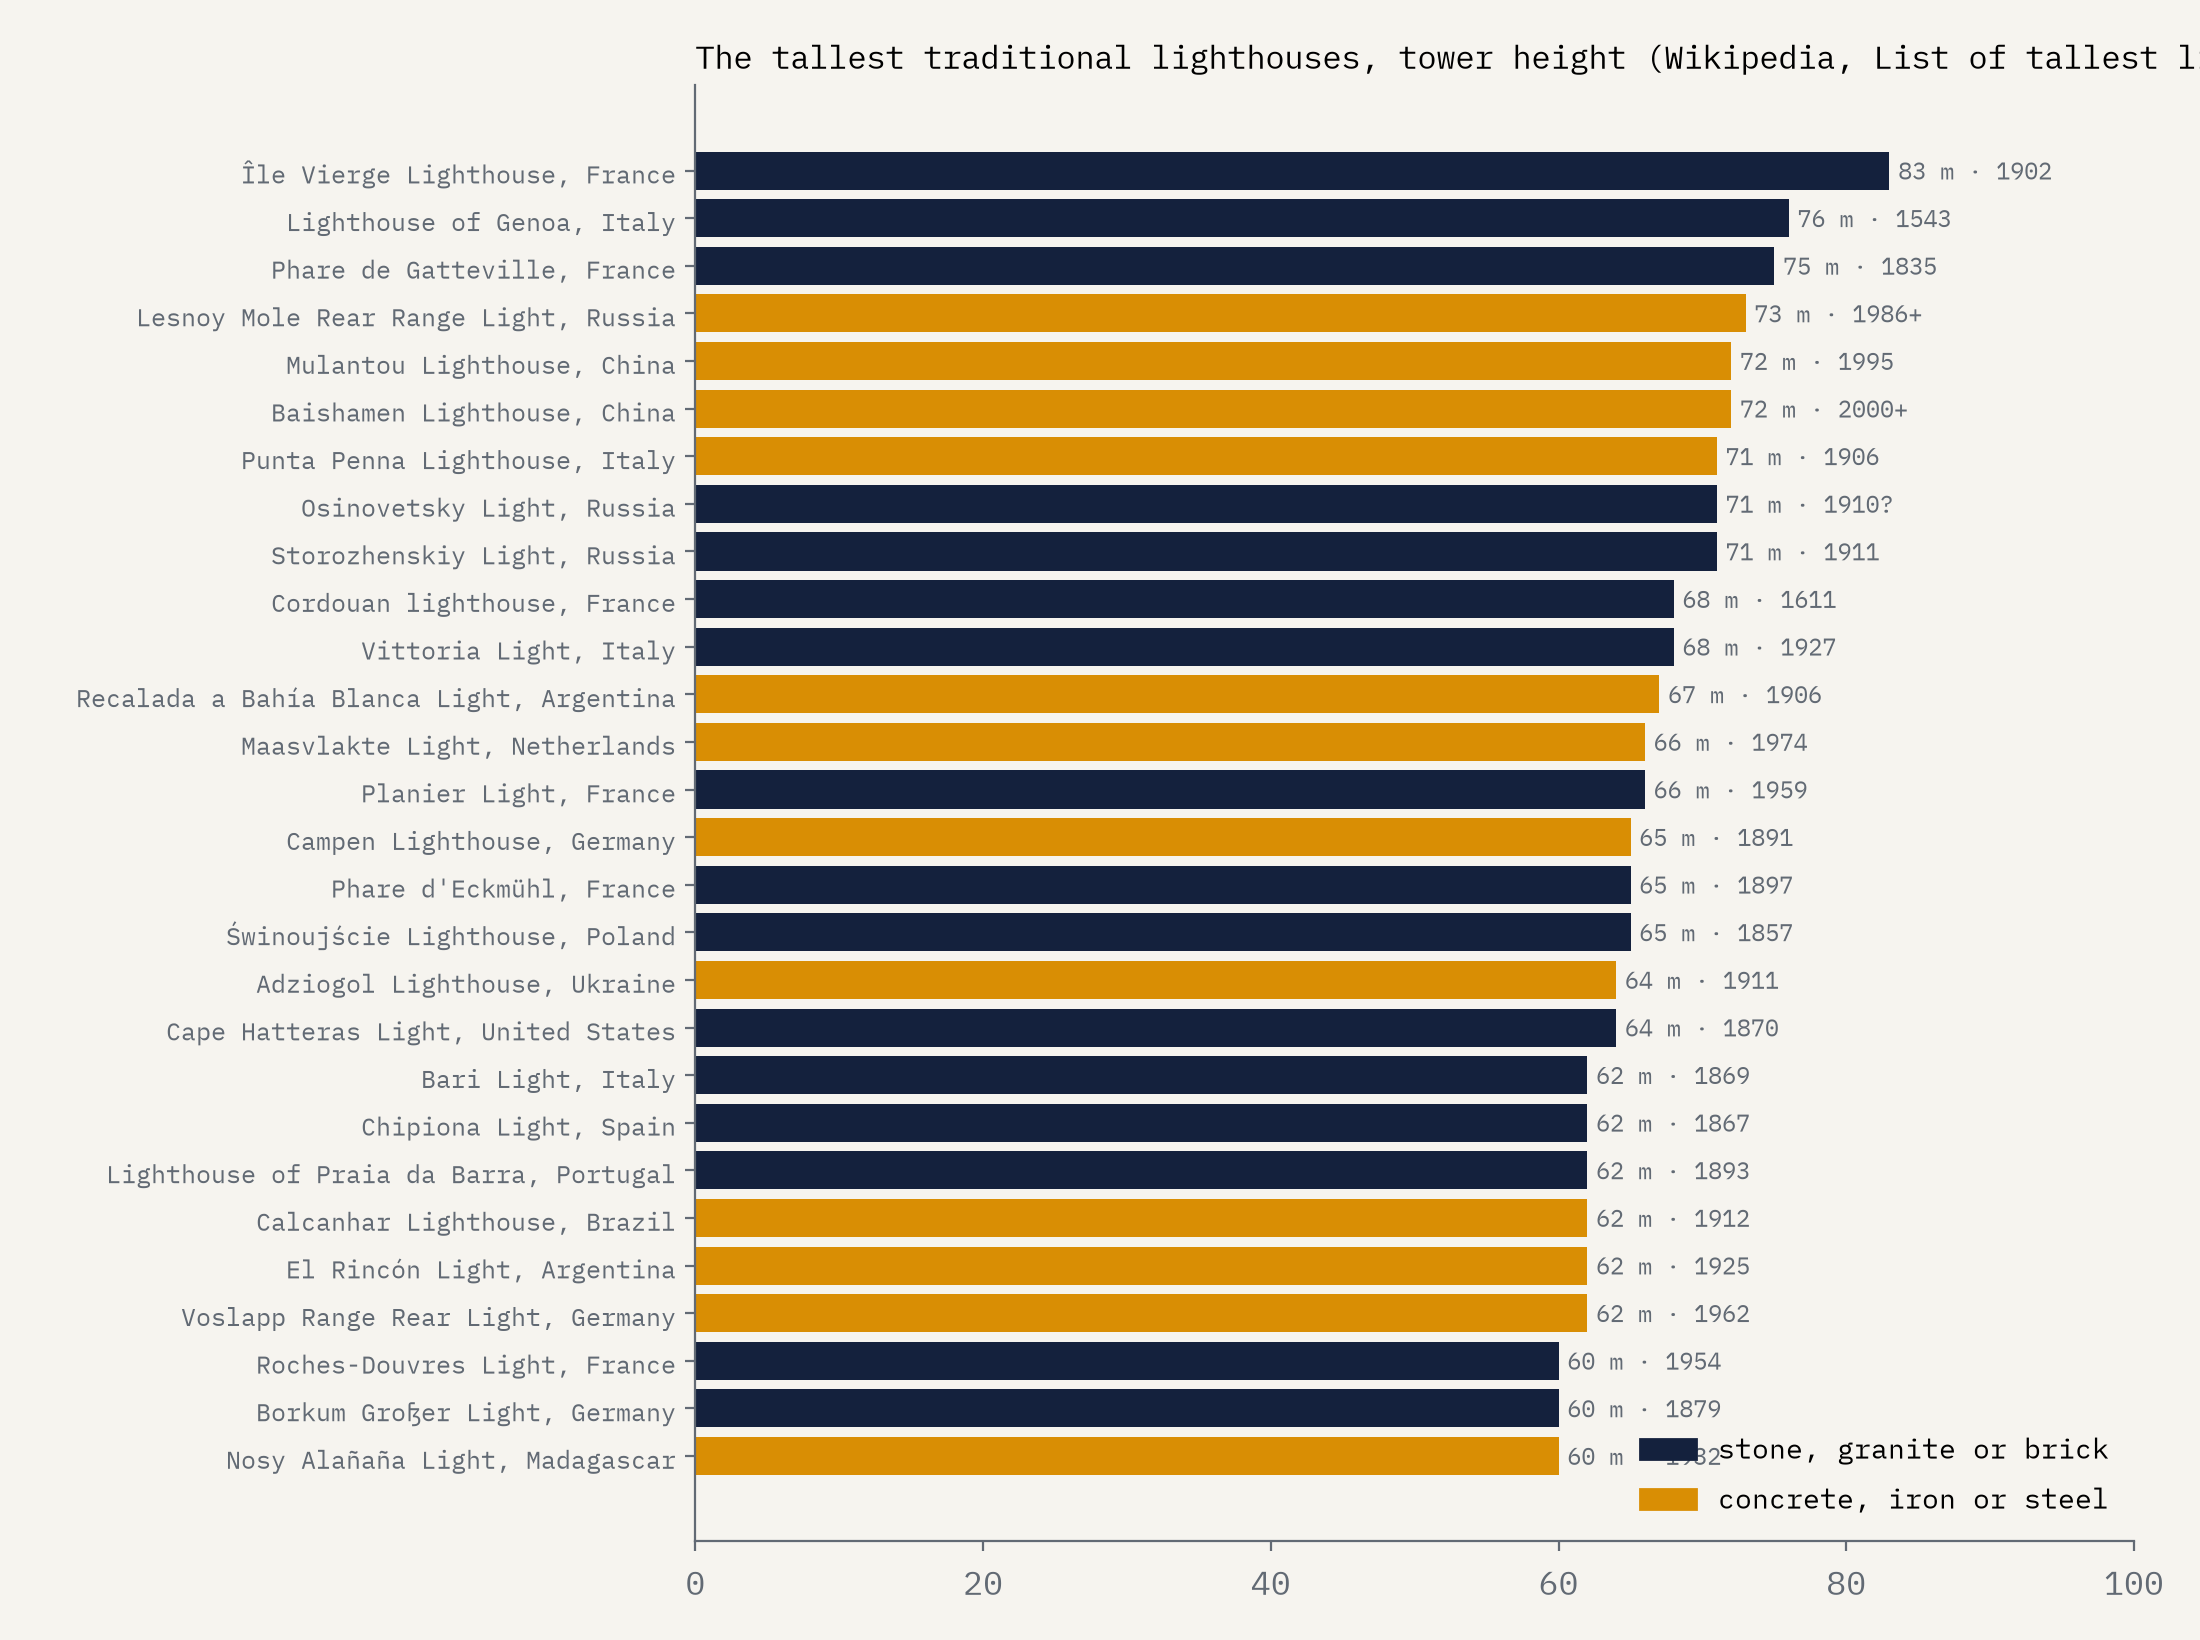
\includegraphics[width=.92\textwidth]{f_tallest.png}
\caption{The tallest traditional lighthouses, from Wikipedia's List of tallest lighthouses.}\label{fig:tallest}\end{figure}

\subsection{Coverage}
5,828 lights (60\%) have at most one Wikipedia article and 4,136 (42\%) have none. The share varies from 0.0\% in Estonia and 16.1\% in the United States to over 90\% in Sweden, Finland and Madagascar (Figure~\ref{fig:coverage}); 970 Swedish and 281 Finnish lights lack an English label, and only 10\% of Finnish lights are dated, against 97\% of Swedish ones. Coastal countries with no lighthouse in Wikidata include Greenland, Nigeria, Kenya, Ecuador and the United Arab Emirates. Europe holds 62\% of all lights, Africa 5\% and South America 3\%.

\begin{figure}[tbp]\centering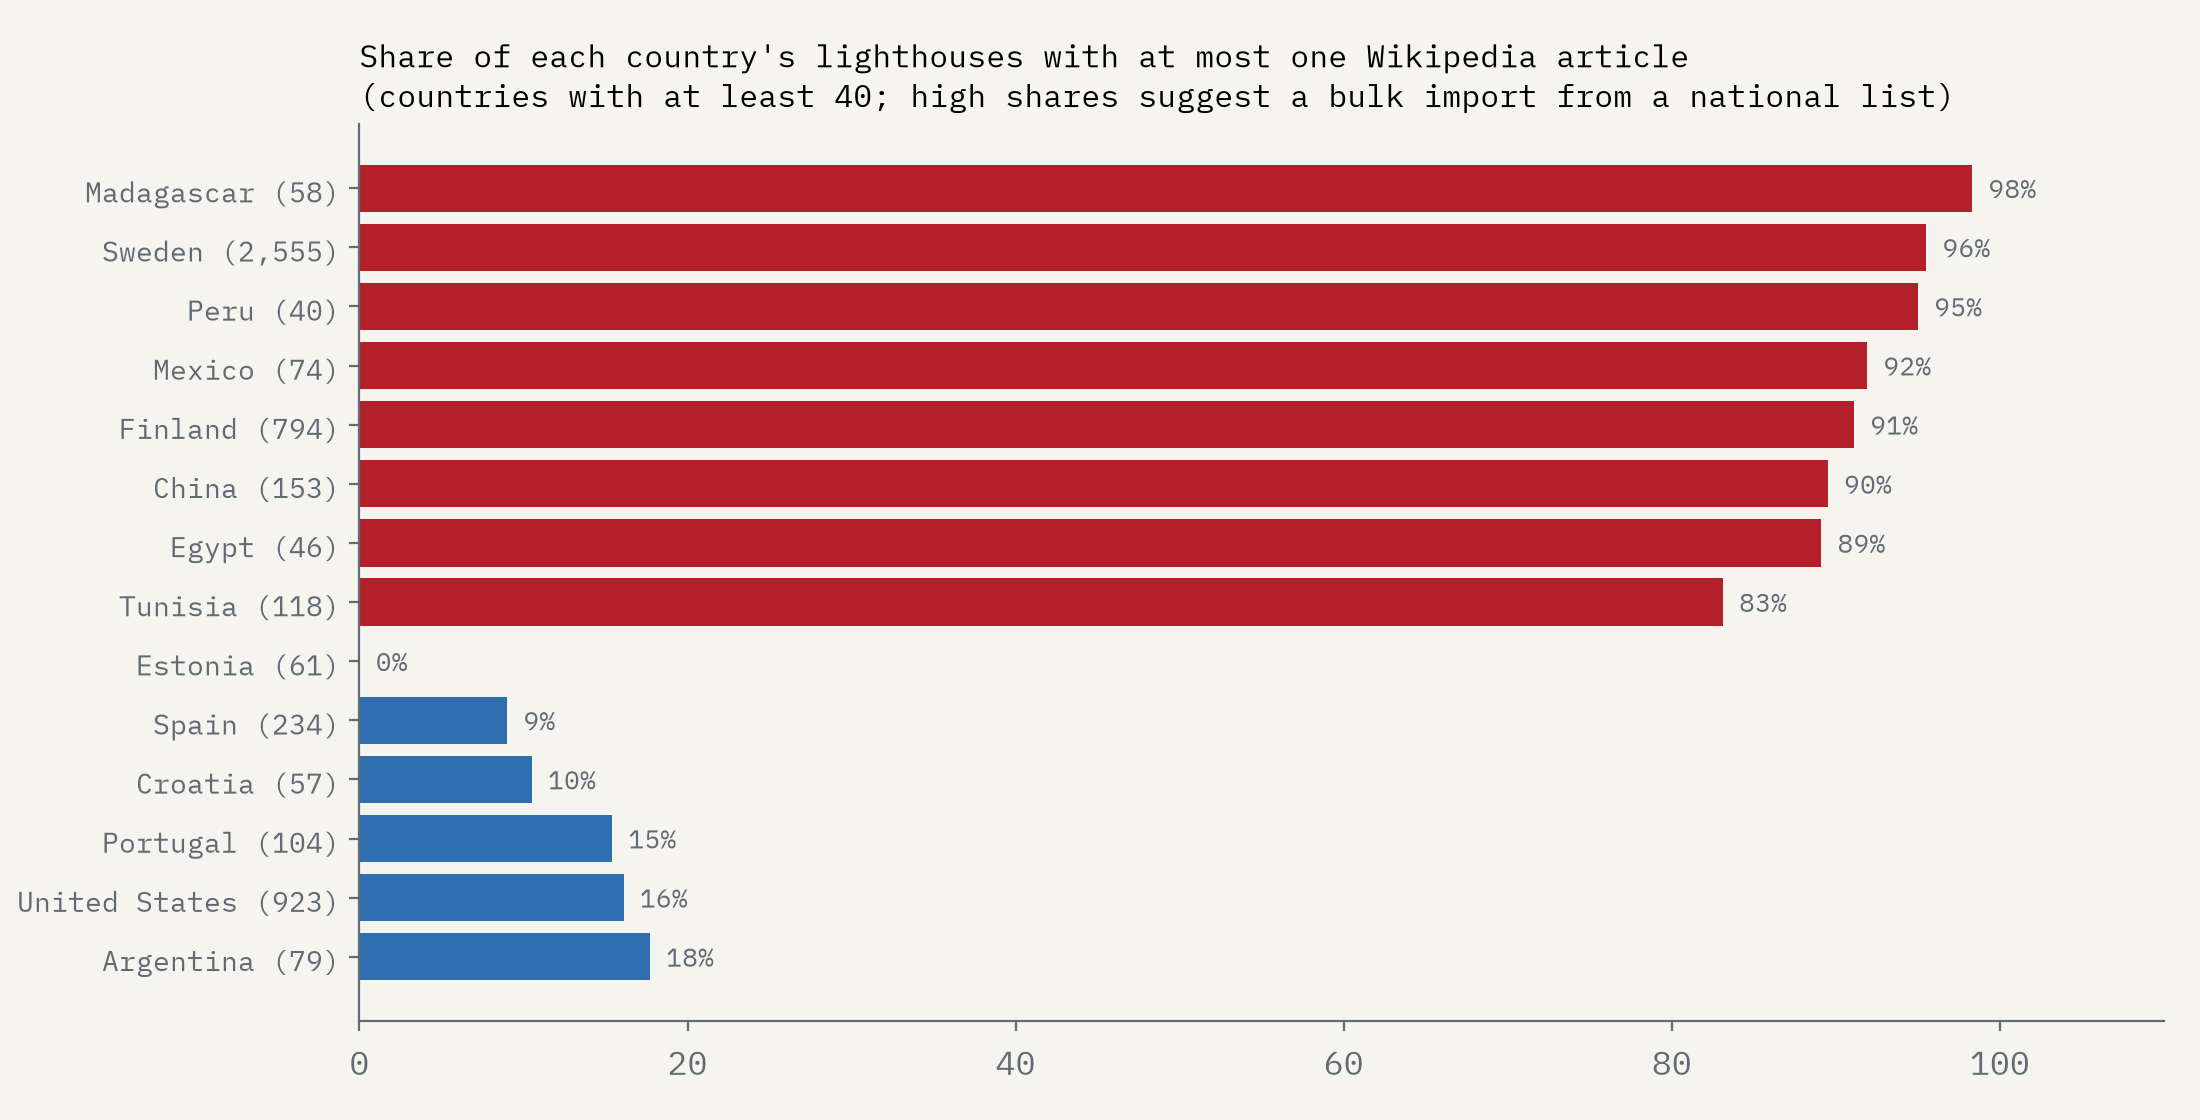
\includegraphics[width=.92\textwidth]{f_coverage.png}
\caption{Share of each country's lighthouses with at most one Wikipedia article (countries with at least 40).}\label{fig:coverage}\end{figure}

\section{Discussion}
The map in Figure~\ref{fig:glow} is two maps laid over each other. One is a map of maritime need: the North Atlantic, the Baltic, the Mediterranean, the coasts of Japan and China and the eastern seaboard of the United States carried the densest shipping of the industrial age and were lit accordingly. The other is a map of the record. Sweden's lights stand out because a national list has been loaded nearly light by light, bare items without articles, often without English names, many of them small twentieth-century lights; Finland and Tunisia show the same signature. Where volunteers add lighthouses one article at a time, as in the United States, Spain or Estonia, records are rich but may stop at the famous towers. Where neither has happened, a coast may appear dark although it is lit.

The timeline is more robust outside Sweden, and its shape, a nineteenth-century rise, a plateau to the First World War and a long decline, fits the history of lighthouse building as it is usually told: the great lighthouse programmes of the Victorian era, the spread of unmanned automatic lights in the twentieth century, the withdrawal of keepers (in the United Kingdom completed in 1998) and the arrival of satellite navigation. It is, though, a timeline of lights that Wikidata knows and dates, by the year it gives, which for old sites is often the first light rather than the present tower.

\section{Limitations}
First, Wikidata is not a register: coverage depends on imports and volunteers and varies by an order of magnitude between countries. Second, inception dates may be the first light, a rebuilding or a rounded century, and items for successive towers on one site sometimes coexist. Third, heights lack units in the extract and are not used for ranking. Fourth, coast lengths are scale dependent and the 1:10m outlines omit many small islands; per-coast densities are comparisons, not absolute measures. Fifth, the sea and inland split uses a simple distance rule, so some estuary and river-mouth lights count as sea lights. Sixth, ``still standing'' was checked by hand for 17 lights only. Finally, the Wikipedia list follows one directory's definition of a traditional lighthouse and leaves out towers such as Jeddah's.

\section{Conclusion}
Put every lighthouse in Wikidata on one map and the coasts of the industrial world light up, with the nineteenth century as the great age of building. Measured against the length of the coast, Scandinavia's lights are the densest, but the brightness of a coast in open data says as much about who has recorded its lights as about the sea. A fuller open register, especially for Africa, South and Southeast Asia and the Pacific, would change the map more than any analysis could.

\section*{Data and code availability}
The interactive map is at \url{https://maps.tristanhotham.com/lighthouses/}. Data and code are at \url{https://github.com/Tristan-Hotham/lighthouses} and archived with this paper at https://doi.org/10.5281/zenodo.23857614. Derived data are released under CC BY 4.0, except the table derived from Wikipedia (CC BY-SA 4.0); code under the MIT licence. Wikidata is CC0; Natural Earth is public domain.

\section*{AI statement}
I wrote the text, with drafting and editing assistance from Claude (Anthropic), which also helped prepare the analysis code. I reviewed and checked all text and results.

\begin{thebibliography}{9}
\bibitem[Mandelbrot(1967)]{mandelbrot} Mandelbrot, B. (1967) How long is the coast of Britain? Statistical self-similarity and fractional dimension. \emph{Science} 156(3775), 636 to 638.
\bibitem[Natural Earth(2026)]{naturalearth} Natural Earth (2026) Admin 0 countries, admin 1 states and provinces, and populated places, 1:10m and 1:50m. Public domain. \url{https://www.naturalearthdata.com/}
\bibitem[Rowlett(2026)]{rowlett} Rowlett, R. (2026) The Lighthouse Directory. University of North Carolina at Chapel Hill. \url{https://www.ibiblio.org/lighthouse/}
\bibitem[Wikidata(2026)]{wikidata} Wikidata (2026) Wikidata, the free knowledge base. CC0. \url{https://www.wikidata.org/}, queried with QLever, \url{https://qlever.cs.uni-freiburg.de/}
\bibitem[Wikipedia(2026)]{wikitall} Wikipedia contributors (2026) List of tallest lighthouses. CC BY-SA 4.0. \url{https://en.wikipedia.org/wiki/List_of_tallest_lighthouses}
\end{thebibliography}
\end{document}
